\documentclass[10pt,a4paper]{article}
\usepackage[utf8]{inputenc}
\usepackage[english]{babel}
\usepackage{amsmath}
\usepackage{amsfonts}
\usepackage{amssymb}
\usepackage{graphicx,float}
\usepackage{subcaption}
\usepackage{float}
\begin{document}
\author{\textbf{Onuray SANCAR}}
\title{\textbf{Experiment 1, The Stefan-Boltzman Radiation Law}}
\date{November 18, 2019}
\maketitle
\textit{with} {\large\textbf{{Yaren AKSEL}}\textit{,} \textbf{Experiment Date}:Novermber 8, 2019\\[3\baselineskip]
\textbf{Abstract}\\[\baselineskip]
The purpose of our experiment is to find the famous Stefan-Boltzman relation. To do this we have first calculated the resistance of our filament, verified the inverse square law and looked for the famous relation both for high and low temperatures. We have found the proportionality constant between the intensity of radiation and the temperature as $2.73\pm0.45$ which is 2.82$\sigma$ away from the real value. \\[\baselineskip]
\textbf{Theory}\\[\baselineskip]
\par The relation between the radiation and temperature had been a hot topic for centuries. There was a definet divergence from a linear behavior as the temperature grew. Josef Stefan introduced a model that stated the relation as $I\propto T^4$, later Boltzmann showed that by treating electromagnetic radiation as the working fluid in a Carnot cycle the $T^4$ law was correct. The law applies only to blackbodies, theoretical surfaces that absord all incident heat radiation.$^{[1]}$
\par The law can be derived from Planck's law by considering a small flat blackbody surface radiating out into a half-sphere.$^{[2]}$
\begin{figure}[H]
	\begin{center}
		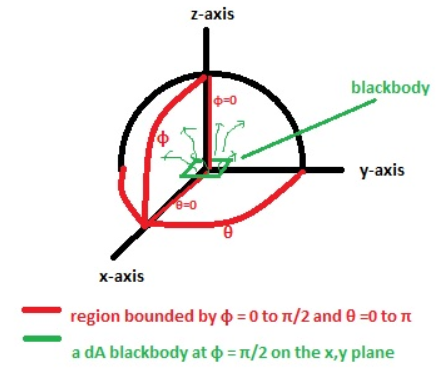
\includegraphics[scale=0.6]{pl.png}
	\end{center}
\end{figure}

\par The intensity of the light emitted from the blackbody surface is given by Planck's law:
\begin{equation}
I\left(\nu ,T\right)=\frac{2h{\nu }^{3}}{{c}^{2}}\frac{1}{{e}^{\frac{h\nu}{kT}}-1}
\end{equation}
where I($\nu$ ,T) is the amount of power per unit surface area per unit solid angle per unit frequency emitted at a frequency $\nu$ emitted by a black body at temperature T, h is Planck's constant, c is speed of light, k is Boltzmann's constant.$^{[2]}$\\
The quantity $I(\nu,T)Ad\nu d\Omega$ is the power radiated by a surface of area A through a solid angle $d\Omega$ in the frequency range between v and v+dv.\\
The Stefan-Boltzmann law gives the power emitted per unit area:
\begin{equation}
\frac{P}{A}=\underset{0}{\overset{\infty }{\int }}I\left(\nu ,T\right)d\nu \int \mathrm{cos}\theta d\Omega
\end{equation}
The cosine appears because black bodies are Lambertian meaning that the intensity observed along the sphere will be the actual intensity times the cosine of the zenith angle.$^{[2]}$
\begin{equation}
\frac{P}{A}=\underset{0}{\overset{\infty }{\int }}I\left(\nu ,T\right)d\nu \underset{0}{\overset{2\pi }{\int }}d\varphi \underset{0}{\overset{\pi/2}{\int }}{\mathrm{cos}}\theta \mathrm{sin}\theta d\theta \\= \pi\underset{0}{\overset{\infty }{\int }}I\left(\nu ,T\right)d\nu
\end{equation} 
\par Making a substitution, $u=\frac{h\nu}{kT}$ and $du=\frac{h}{kT}d\nu$
\begin{equation}
\frac{P}{A}=\frac{2\pi h}{{c}^{2}}{\left(\frac{kT}{h}\right)}^{4}\underset{0}{\overset{\infty }{\int }}\frac{{u}^{3}}{{e}^{u}-1}du
\end{equation}
\par Which gives
\begin{equation}
\frac{P}{A}=\sigma T^4, \sigma=\frac{2\pi^5k^4}{15c^2h^3}.
\end{equation}
\textbf{Apparatus}
\\[\baselineskip]
\begin{itemize}
	\item \textbf{Stefan-Bolztman Lamp}: Used as radiation source in first parts of the experiment.
	\item \textbf{Ammeter}: Used to measure the current in the system.
	\item \textbf{Voltmeter}: Used to measure the voltage in the system.
	\item \textbf{Electrical Oven}: Used to increase temperature steadily in the last part of the experiment.
	\item \textbf{Temperature Probe with Display}: Used to measure temperature.
	\item \textbf{Radiation Sensor}: Read radiation is turned to voltage through means.
	\item \textbf{Ruler}: Used to measure distance between between the lamp and the radiation sensor.
	\item \textbf{Multimeters}: Used to measure/apply smaller values of voltages and currents than otherwise possible.
	\item \textbf{Voltage Amplifier}: Used to amplify low voltage.
	\\[\baselineskip]
\end{itemize}
\textbf{Procedure}
\\[\baselineskip]
\begin{enumerate}
	\item We connected radiation sensor and the Stefan-Boltzman lamp to voltmeter and a power source respectively.
	\item We have adjusted our read values to get rid of the effects of background but at some range the voltmeter did not work the way we wanted so we did not direclty see the effects of the background radiation.
	\item We have connected multimeters to the set-up and then applied voltage at 0-20mV range. We have measured the resistance from these voltages and measured voltage from the sensor.
	\item Inverse Square Law Part: We have created a substantial radiation from the lamp then have taken datas at different distances from the sensor to see the inverse square law in the sensor voltage region of $3\times 10^{-2}$V and $10^{-3}$V.
	\item High temperature part: We have measured the output voltage at the 3 different distances between the lamp and the sensor. We have applied various different voltages and currents.
	\item Low temperature part: By using an electrical oven we have increased temperature of our system and measured the voltage output in our sensor. We have placed the sensor to an appropriate distance from the oven and also we placed a shielding between them to reduce reflections. We collected data up to 400$^oC$.
	\\[\baselineskip]
\end{enumerate}
\textbf{Data}\\[\baselineskip]
\par Table 12.1 Temperature and Resistivity as a function of the Relative resistance of the Tungsten filament
\begin{figure}[H]
	\begin{center}
		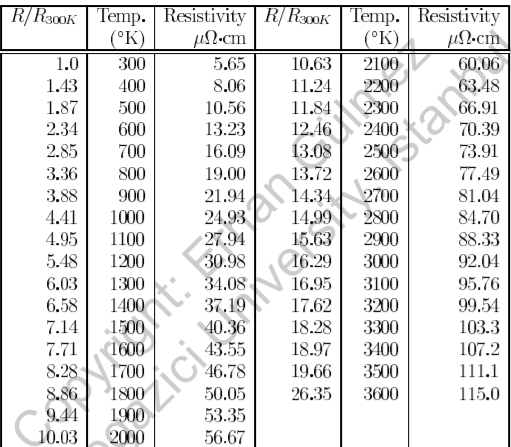
\includegraphics[scale=0.7]{table.png}
	\end{center}
\end{figure}
\begin{center}
	\begin{figure} [H] 
		\begin{tabular}{|c |c||c|c|} \hline
			Potential Difference (mV)& Current (mA) & Potential Difference (mV)& Current (mA)\\ [0.5ex] 
			\hline
			0.8 & 2.75 & 9.2 &31.31\\
			\hline
			1.0 & 3.53 &9.9 & 33.73\\
			\hline 
			1.7 & 5.76 & 12.6 & 42.90\\
			\hline 
			2.3 & 7.40 & 14.5 & 49.40\\
			\hline 
			4.1 & 14.09 & 16.4 & 55.70\\
			\hline 
			5.5 & 18.66 & 17.8 & 6.40\\
			\hline 
			7.4 & 25.23 & 19.5 & 66.60\\
			\hline
		\end{tabular}
		\caption{Data for initial part of the experiment. Errors for potential difference is 0.1mV and the error for the current is 0.01mA. }
	\end{figure}
\end{center}
\begin{center}
	\begin{figure} [H] 
		\begin{tabular}{|c |c||c|c|} \hline
			Potential Difference (V)& Distance (cm) & Potential Difference (V)& Distance (cm)\\ [0.5ex] 
			\hline
			0.45$\times10^{-2} \pm 0.05\times10^{-2}$ & 3.0$\pm0.1$ & 0.9$\times10^{-3} \pm 0.05\times10^{-3}$ &11.0$\pm0.1$\\
			\hline
			0.35$\times10^{-2} \pm 0.05\times10^{-2}$ & 4.0$\pm0.1$&0.85$\times10^{-3} \pm 0.05\times10^{-3}$ & 11.5$\pm0.1$\\
			\hline 
			0.25$\times10^{-2} \pm 0.05\times10^{-2}$ & 5.0$\pm0.1$ & 0.75$\times10^{-3} \pm 0.05\times10^{-3}$ &12.0$\pm0.1$\\
			\hline 
			0.20$\times10^{-2} \pm 0.05\times10^{-2}$ & 6.0$\pm0.1$ & 0.7$\times10^{-3} \pm 0.05\times10^{-3}$ & 13.0$\pm0.1$\\
			\hline 
			1.8$\times10^{-3} \pm 0.2\times10^{-3}$ & 7.0$\pm0.1$ &  & \\
			\hline 
			1.6$\times10^{-3} \pm 0.2\times10^{-3}$ & 7.5$\pm0.1$ &  &\\
			\hline 
			1.4$\times10^{-3} \pm 0.2\times10^{-3}$ & 8.0$\pm0.1$ &   & \\
			\hline
			1.4$\times10^{-3} \pm 0.2\times10^{-3}$&8.5$\pm0.1$& &\\
			\hline
			1.2$\times10^{-3} \pm 0.2\times10^{-3}$&9.0$\pm0.1$& &\\
			\hline
			1.0$\times10^{-3} \pm 0.2\times10^{-3}$&10.0$\pm0.1$& &\\
			\hline
		\end{tabular}
		\caption{Data for the inverse square law part of the experiment with 0.9V of applied voltage and 2.3A of applied current.}
	\end{figure}
\end{center}
\begin{center}
	\begin{figure} [H] 
		\begin{tabular}{|c |c|c|} \hline
			Applied Potential Difference (V)& Applied Current(A) & Measured Potential Difference (V)\\ [0.5ex] 
			\hline
			6.77 & 2.232 & 1.8$\times10{-3}$\\
			\hline
			7.15 & 2.287 & 2.2$\times10{-3}$\\
			\hline
			5.60 & 2.015 & 1.4$\times10{-3}$\\
			\hline
			3.93 & 1.688 & 0.8$\times10{-3}$\\
			\hline
			3.088 & 1.509 & 0.6$\times10{-3}$\\
			\hline
		\end{tabular}
		\caption{Data for the high temperature part of the experiment for distance between the lamp and the sensor 5.4$\pm0.1$cm.The uncertainty in applied voltage is 0.01 Volts, The uncertainty in applied current is 0.001 Ampere and the uncertainty in measured voltage is 0.0001 Volts.}
	\end{figure}
\end{center}
\begin{center}
	\begin{figure} [H] 
		\begin{tabular}{|c |c|c|} \hline
			Applied Potential Difference (V)& Applied Current(A) & Measured Potential Difference (V)\\ [0.5ex] 
			\hline
			3.511 & 1.601 & 0.4$\times10{-3}$\\
			\hline
			5.45 & 1.995 & 0.8$\times10{-3}$\\
			\hline
			6.40 & 2.162 & 1.0$\times10{-3}$\\
			\hline
			7.14 & 2.285 & 1.2$\times10{-3}$\\
			\hline
			7.75 & 2.386 & 1.4$\times10{-3}$\\
			\hline
		\end{tabular}
		\caption{Data for the high temperature part of the experiment for distance between the lamp and the sensor 8.4$\pm0.1$cm.The uncertainty in applied voltage is 0.01 Volts, The uncertainty in applied current is 0.001 Ampere and the uncertainty in measured voltage is 0.0001 Volts.}
	\end{figure}
\end{center}
\begin{center}
	\begin{figure} [H] 
		\begin{tabular}{|c |c|c|} \hline
			Applied Potential Difference (V)& Applied Current(A) & Measured Potential Difference (V)\\ [0.5ex] 
			\hline
			7.76 & 2.386 & 0.8$\times10{-3}$\\
			\hline
			7.09 & 2.274 & 0.8$\times10{-3}$\\
			\hline
			8.22 & 2.458 & 1.0$\times10{-3}$\\
			\hline
			5.94 & 2.075 & 0.6$\times10{-3}$\\
			\hline
			4.64 & 1.832 & 0.4$\times10{-3}$\\
			\hline
		\end{tabular}
		\caption{Data for the high temperature part of the experiment for distance between the lamp and the sensor 11.4$\pm0.1$cm.The uncertainty in applied voltage is 0.01 Volts, The uncertainty in applied current is 0.001 Ampere and the uncertainty in measured voltage is 0.0001 Volts.}
	\end{figure}
\end{center}
\begin{center}
	\begin{figure} [H] 
		\begin{tabular}{|c |c||c|c|} \hline
			Temperature($^oC$)& Potential Difference(V) & Temperature($^oC$) & Potential Difference(V)\\ [0.5ex] 
			\hline
			29.5 $\pm0.1$ & 0.05$\times10{-3}$ & 79.5$\pm0.1$ &1.2$\times10{-3}$\\
			\hline
			31.1 $\pm0.1$ & 0.1$\times10{-3}$ &85.5$\pm0.1$ & 1.4$\times10{-3}$\\
			\hline 
			33.5 $\pm0.1$ & 0.15$\times10{-3}$ & 93.6$\pm0.1$ & 1.6$\times10{-3}$\\
			\hline 
			36.0  $\pm0.1$& 0.20$\times10{-3}$ & 100.0$\pm0.1$ &1.8$\times10{-3}$\\
			\hline 
			38.3$\pm0.1$ & 0.25$\times10{-3}$ & 112.8$\pm0.1$ & 2.2$\times10{-3}$\\
			\hline 
			41.3$\pm0.1$ & 0.30$\times10{-3}$ & 124.3$\pm0.1$ & 2.6$\times10{-3}$\\
			\hline 
			43.9$\pm0.1$ & 0.35$\times10{-3}$ & 139.4$\pm0.1$ & 3.0$\times10{-3}$\\
			\hline
			45.6$\pm0.1$ & 0.40$\times10{-3}$ & 162.7$\pm0.1$ & 4.0$\times10{-3}$\\
			\hline
			48.4$\pm0.1$ & 0.45$\times10{-3}$ & 203.7$\pm0.1$ & 6.0$\times10{-3}$\\
			\hline
			50.8$\pm0.1$ & 0.50$\times10{-3}$ & 220.4$\pm0.1$ & 7.0$\times10{-3}$\\
			\hline
			53.3$\pm0.1$ &0.55$\times10{-3}$ & 236.5$\pm0.1$  & 8.0$\times10{-3}$\\
			\hline
			55.8$\pm0.1$ &0.60$\times10{-3}$ & 252.3$\pm0.1$  & 9.0$\times10{-3}$\\
			\hline
			58.0$\pm0.1$ &0.65 $\times10{-3}$ & 303.6$\pm0.1$ & 14.0$\times10{-3}$\\
			\hline
			62.8$\pm0.1$ &0.75$\times10{-3}$ & 342.4$\pm0.1$  & 18.0$\times10{-3}$\\
			\hline
			64.4$\pm0.1$ &0.80$\times10{-3}$ & 374.8$\pm0.1$ &  22.0$\times10{-3}$\\
			\hline
			69.1$\pm0.1$ &0.90$\times10{-3}$ &        &             \\
			\hline
		\end{tabular}
		\caption{Data for the low temperature part of the experiment.Errors for potential difference are 0.01$\times10{-3}$ for the left part and 0.1$\times10{-3}$ for the right part.}
	\end{figure}
\end{center}
s
\\[\baselineskip]
\textbf{Analysis}\\[\baselineskip]
\par Some useful formulas:
\par Error propagation
\begin{equation}
{\sigma }_{f}=\sqrt{\sum _{i}^{n}{\left(\frac{\partial f}{\partial {x}_{i}}\right)}^{2}{\sigma }_{{x}_{i}}^{2}+\dots }
\end{equation}
\par Weighted average
\begin{equation}
f_{weighted}=\frac{\sum _{i}\frac{{f}_{i}}{{\sigma_i }^{2}}}{\sum _{i}\frac{1}{{\sigma_i }^{2}}}
\end{equation}
\par Where $\sigma_i$ is the uncertainty in $f_i$
\par By taking the weighted sum of the $R_{300}=voltage/current$ we get $R_{300}$ (the error in $R_{300}$ is not written because it is not needed for rest of the analysis)
\begin{equation}
R_{300}=\frac{\sum _{i}\frac{{R}_{i}}{{\sigma_i }^{2}}}{\sum _{i}\frac{1}{{\sigma_i }^{2}}}=0.2938\Omega
\end{equation}
\par We have used the table's datas, given in the book, to fit a line to the graph of temperature vs. R/$R_{300}$. This way we can convert the resistance we have found in the later parts of the experiment to the corresponding temperature. There is no errorbar in this graph because the values are taken as given. 
\begin{figure}[H]
\advance\leftskip1.25cm
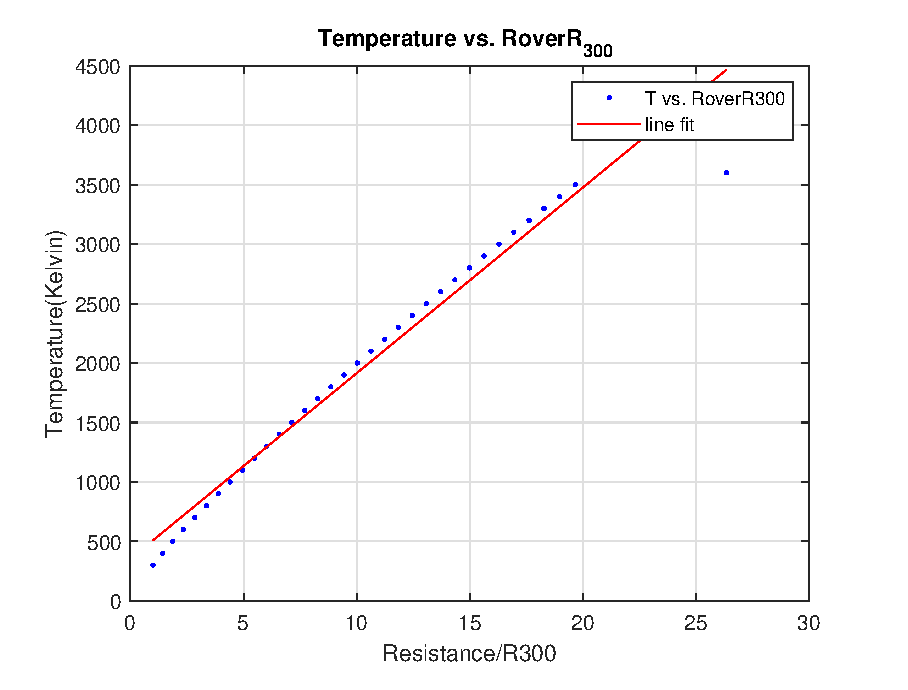
\includegraphics[scale=0.7]{RR.eps}
\caption{$f(x) = p_1x^{-2}+p_2$ with $p_1=156.2 \pm10.3$, $p_2=352.8\pm122.3$. R-square=0.9679}
\end{figure}
\par For the inverse square law part we first fit a polynomial to see look fo what to do next.
\begin{figure}[H]
	\advance\leftskip1.25cm
	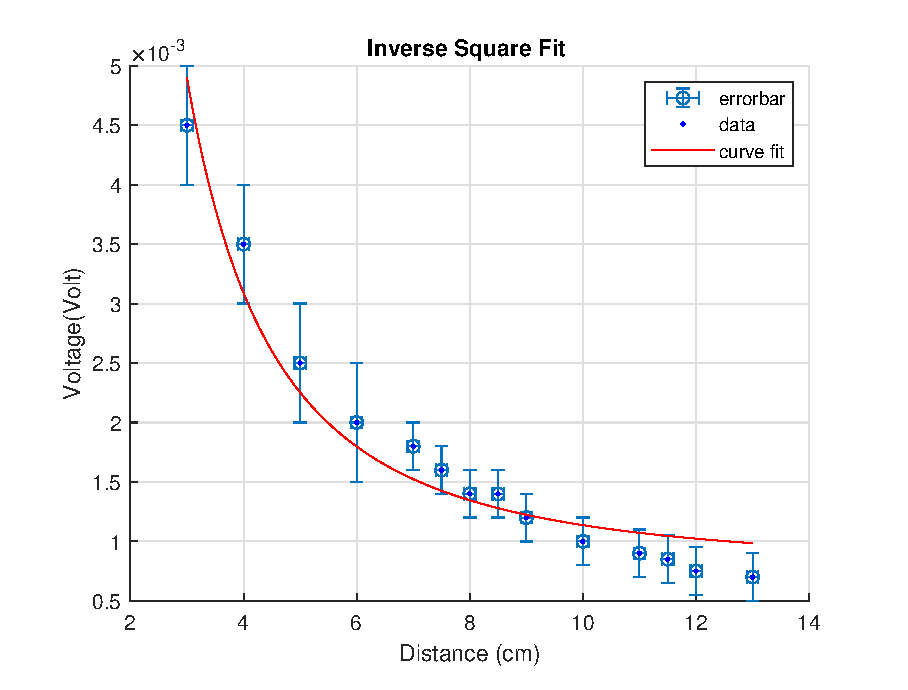
\includegraphics[scale=0.7]{ISL.eps}
	\caption{$f(x) = p_1x^{-2}+p_2$ with $p_1=0.0372 \pm0.0054$, $p_2=0.0007646\pm0.0002035$. R-square=0.9503}	
\end{figure}
\par We create log-log graph for the inverse square fit so we can see the relation between the read voltage(intesity) and the distance.
\begin{figure}[H]
	\advance\leftskip1.25cm
	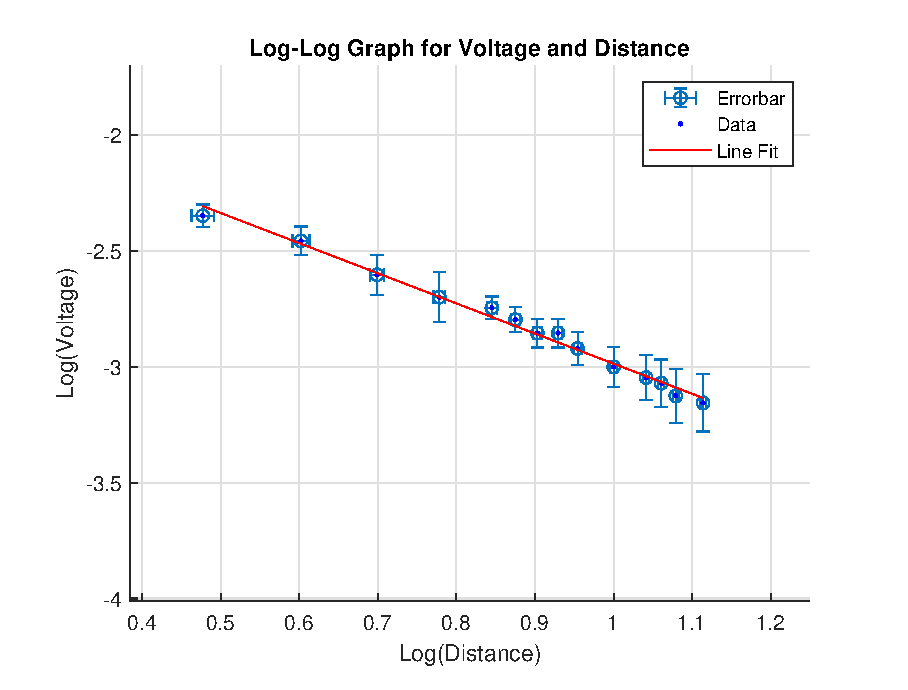
\includegraphics[scale=0.7]{ISLlog.eps}	
	\caption{$f(x) = p_1x+p_2$ with $p_1=-1.301 \pm0.082$, $p_2=-1.685\pm0.075$. R-square=0.9899}
\end{figure}
\par We have found the proportionality constant n in $I\propto D^n$ as $-1.301 \pm0.082$ which is 8.5$\sigma$ away from the real value.
\par By using the temperature vs. R/$R_{300}$ fit, we have obtained the Log(Voltage) vs. Log(Temperature) using the data for the d=5.4cm part:
\begin{figure}[H]
\advance\leftskip1.25cm
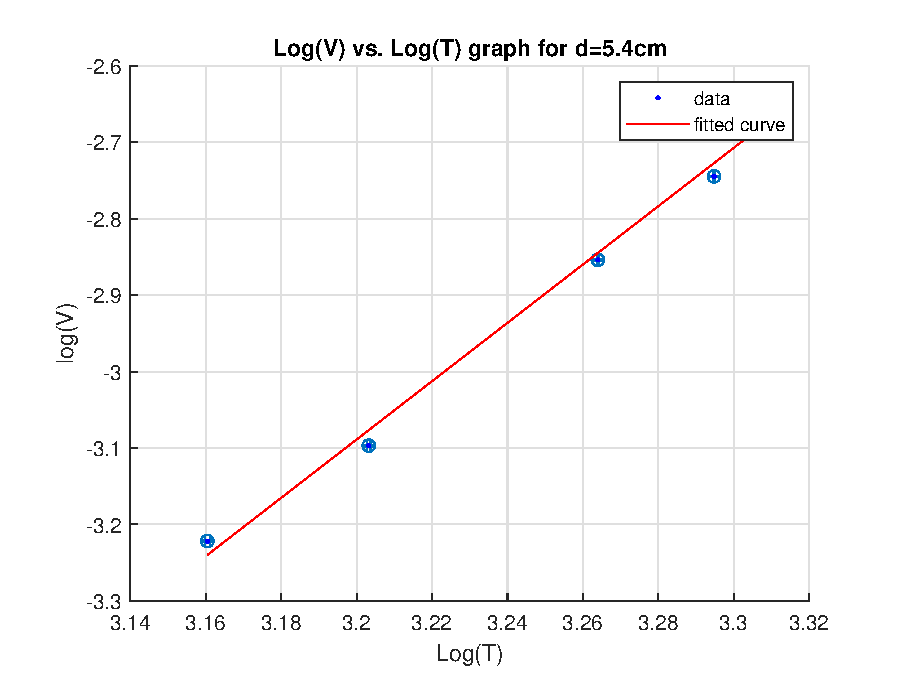
\includegraphics[scale=0.7]{d1high.eps}
\caption{$f(x) = p_1x+p_2$ with $p_1=5.742\pm0.871$, $p_2=-19.5\pm2.5$. R-square=0.9932}
\end{figure}
\par From this graph we see the proportionality constant n in $I\propto T^n$ as $n=5.742\pm0.871$. 
\par By using the temperature vs. R/$R_{300}$ fit, we have obtained the Log(Voltage) vs. Log(Temperature) using the data for the d=8.4cm part:
\begin{figure}[H]
\advance\leftskip1.25cm
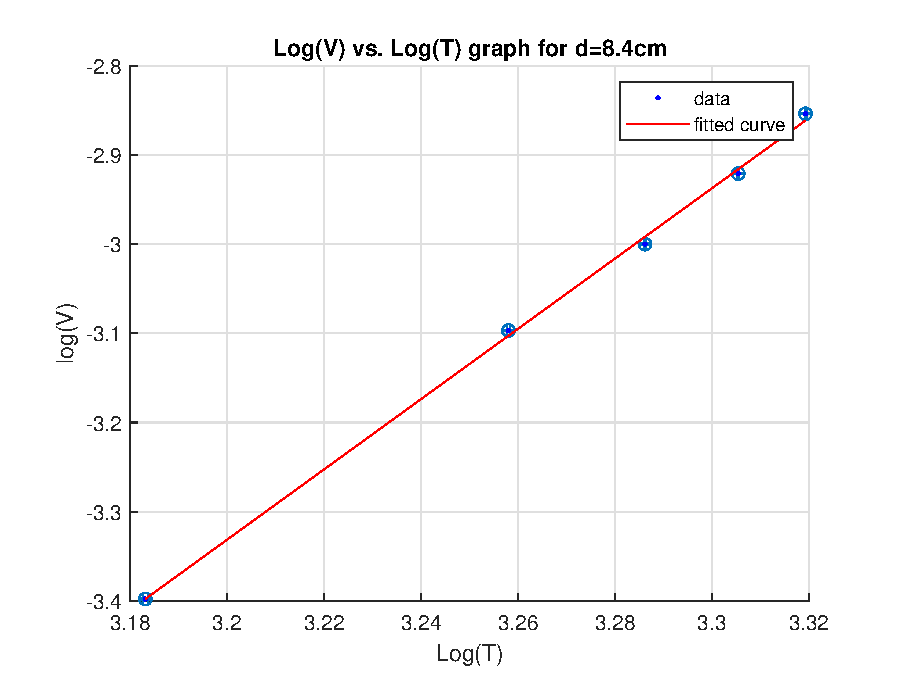
\includegraphics[scale=0.7]{d2high.eps}
\caption{$f(x) = p_1x+p_2$ with $p_1=5.859 \pm0.349$, $p_2=-20.07\pm1.01$. R-square= 0.999}
\end{figure}
\par From this graph we see the proportionality constant n in $I\propto T^n$ as $n=5.859 \pm0.349$.
\par By using the temperature vs. R/$R_{300}$ fit, we have obtained the Log(Voltage) vs. Log(Temperature) using the data for the d=11.4cm part:
\begin{figure}[H]
\advance\leftskip1.25cm
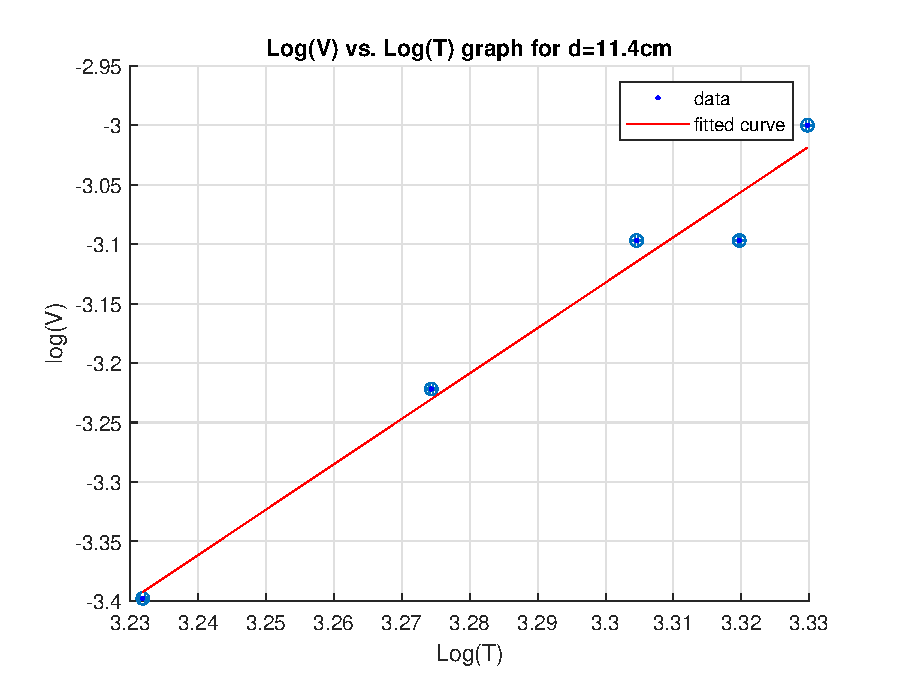
\includegraphics[scale=0.7]{d3high.eps}
\caption{$f(x) = p_1x+p_2$ with $p_1=5.543 \pm1.655$, $p_2=-19.34\pm4.83$. R-square= 0.9743}
\end{figure}
\par From this graph we see the proportionality constant n in $I\propto T^n$ as $n=5.543 \pm1.655$.
\par By taking their weighted average we get:
\begin{equation}
n_{weighted}=5.832\pm0.338
\end{equation}
\par First we transform our Celsius datas to Kelvins by just adding 273.15 to Celsius datas. Then we fit a line to log(Voltage) vs. log(Temperature) graph to see the behavior at lower temperatures.
\begin{figure}[H]
\advance\leftskip1.25cm
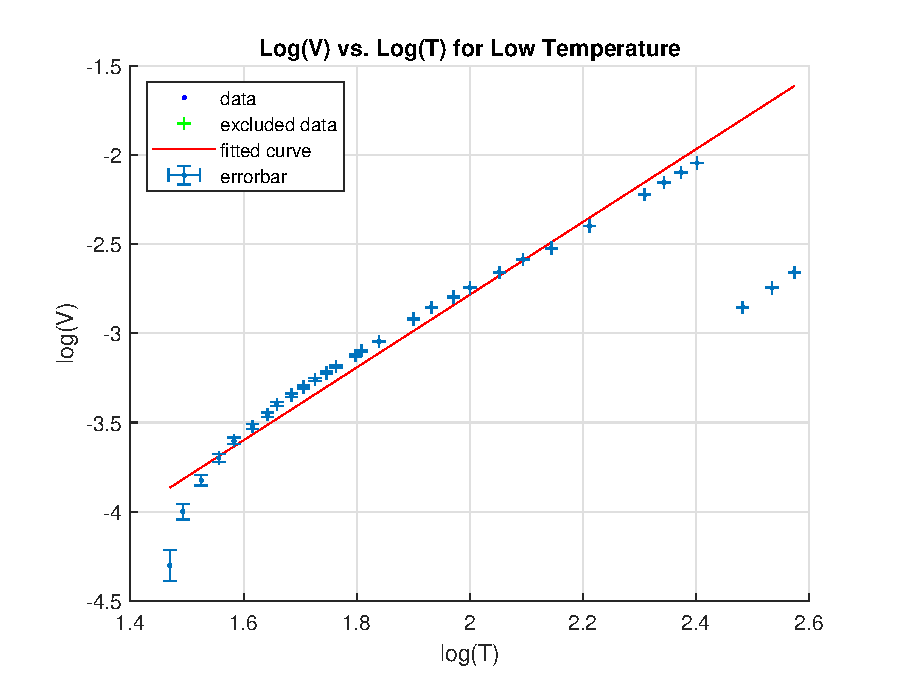
\includegraphics[scale=0.7]{lowtemp.eps}
\caption{$f(x) = p_1x+p_2$ with $p_1=2.04\pm0.16$, $p_2=-6.864\pm0.298$. R-square=0.9633}
\end{figure}
\par From this graph we see the proportionality constant n in $I\propto T^n$ as $n=2.04\pm0.16$ for lower temperatures.
\par Taking weighted averages of part 2 and part 3 we get:
\begin{equation}
n_{weighted}=2.73\pm0.45
\end{equation}
\par We have found the proportionality constant  2.82$\sigma$ away from the expected value, 4.
\\[\baselineskip]
\textbf{Conclusion}
\\[\baselineskip]
\par The proportionality constant we have found is not that close to the real value. But this was to be expected. We were not really careful about some parts of the experiment. We sometimes lean over to the lamp's side differing the value read by the sensor. Also the reflective surface all around the setup might have caused some problems. For low temperature part the electric oven was not examined beforehand so this might have caused a problem in that part. For the same reasons stated earlier the inverse square law part came as terrible. To improve these, we can isolate our setup from the background and human interventions and cover it with nonreflective surfaces; and the electric oven can be replaced with a new one.
\\[\baselineskip] \textbf{References}\\[\baselineskip]
\par[1]A Brief History of the $T^4$ Radiation Law - Crepeau, John. 
\par https://pdfs.semanticscholar.org/748d/6a04e78f8dd3bdc15bdb74365e1a9db0667d.pdf 
\par[2]Wikipedia, Stefan-Boltzmann Law.
\par[3]Advanced Physics Experiments - Gülmez, Prof. Dr. Erhan.
\\[\baselineskip] \textbf{Appendix}\\[\baselineskip]
\par The non logartihmic graphs of some parts that was not needed in the analysis:
\begin{figure}[H]
	\advance\leftskip1.25cm
	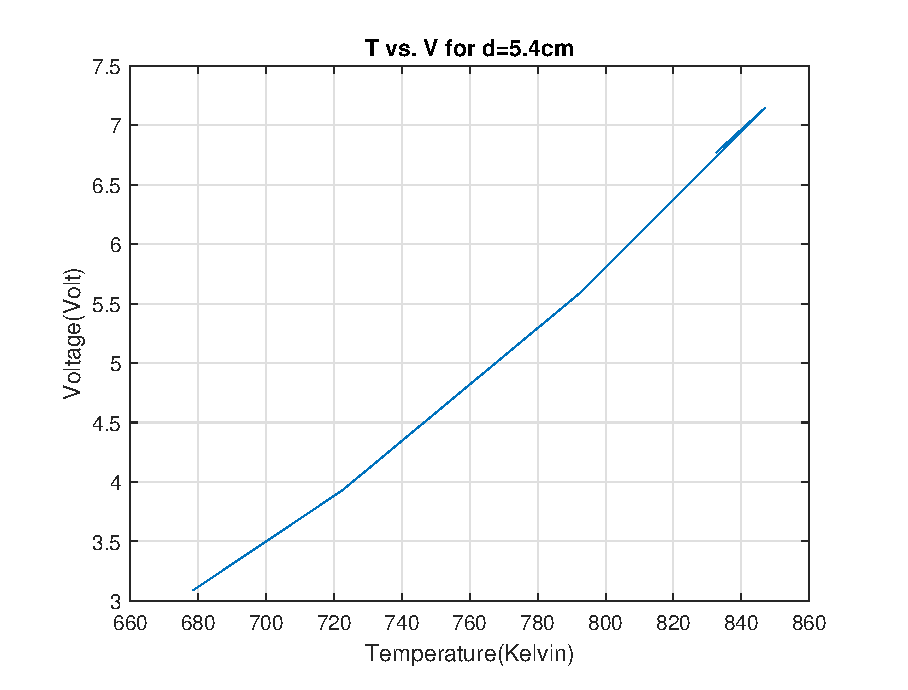
\includegraphics[scale=0.7]{5notneeded.eps}
	
\end{figure}
\begin{figure}[H]
	\advance\leftskip1.25cm
	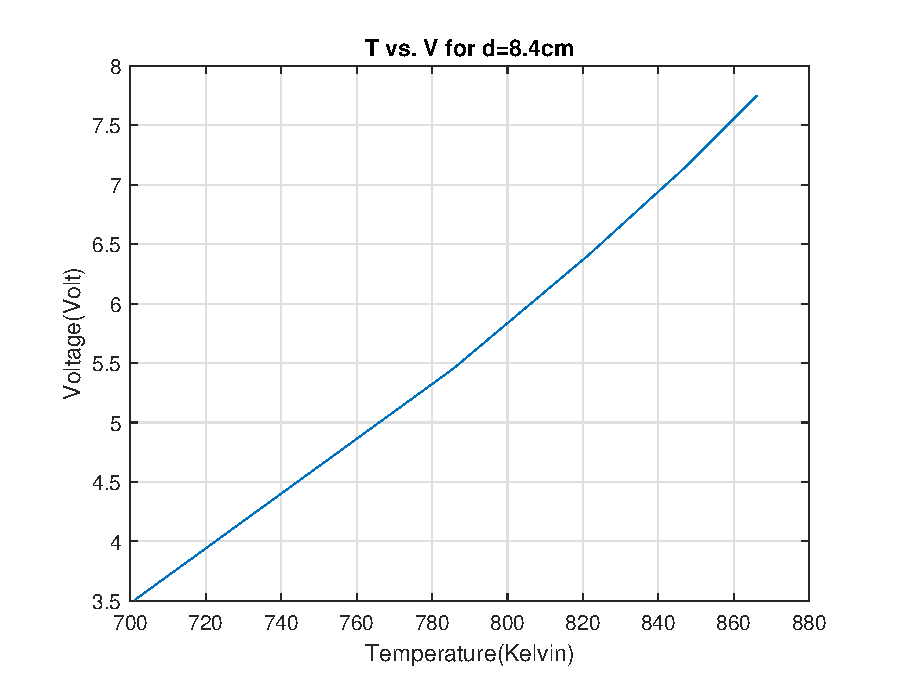
\includegraphics[scale=0.7]{8notneeded.eps}
	
\end{figure}
\begin{figure}[H]
	\advance\leftskip1.25cm
	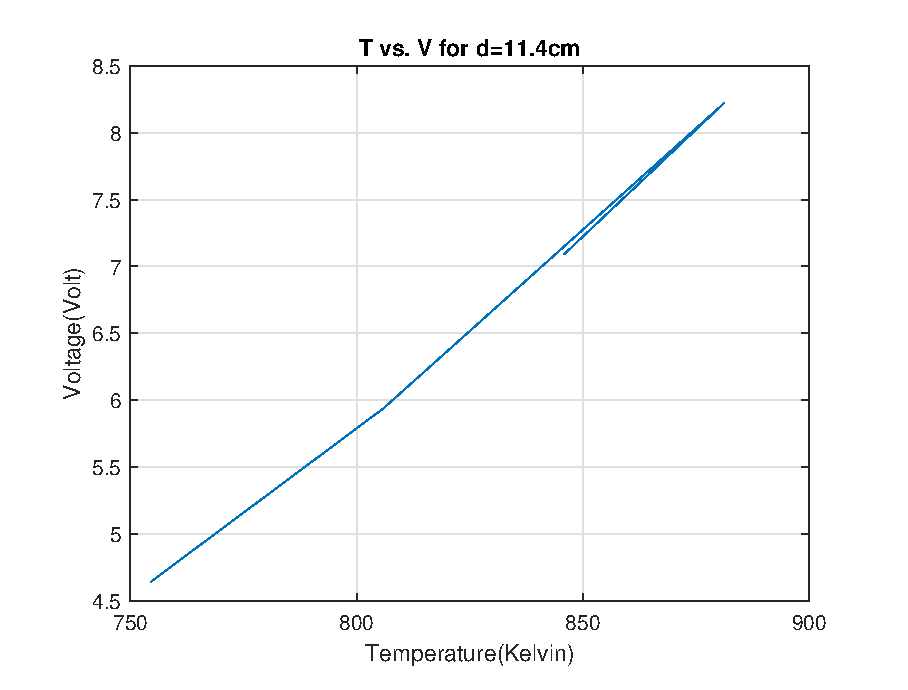
\includegraphics[scale=0.7]{11notneeded.eps}
	
\end{figure}
\begin{figure}[H]
	\advance\leftskip1.25cm
	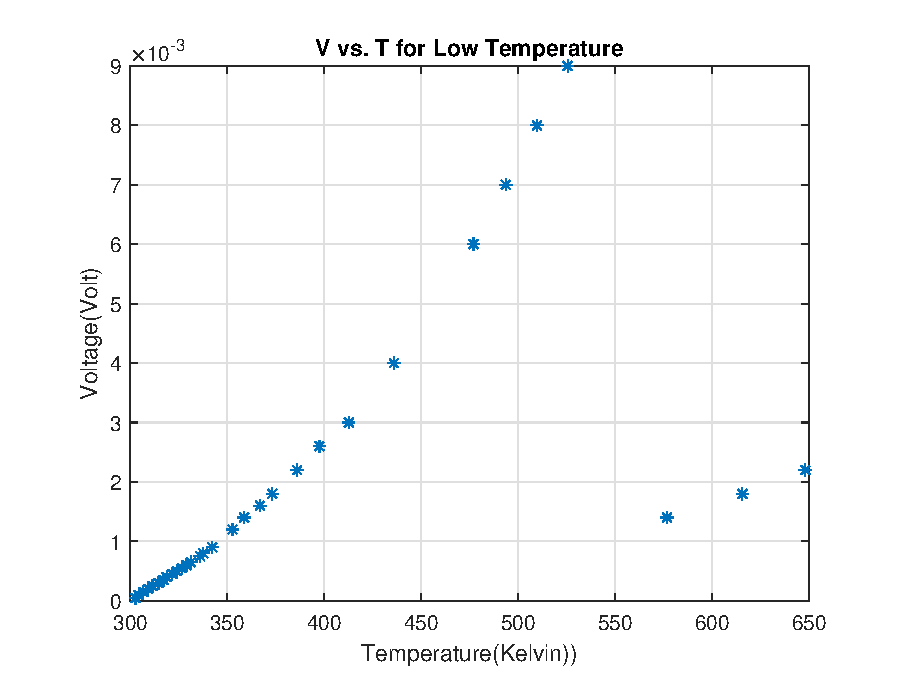
\includegraphics[scale=0.7]{Tnotneeded.eps}
	
\end{figure}
\end{document}